\documentclass[]{article}
\usepackage{lmodern}
\usepackage{amssymb,amsmath}
\usepackage{ifxetex,ifluatex}
\usepackage{fixltx2e} % provides \textsubscript
\ifnum 0\ifxetex 1\fi\ifluatex 1\fi=0 % if pdftex
  \usepackage[T1]{fontenc}
  \usepackage[utf8]{inputenc}
\else % if luatex or xelatex
  \ifxetex
    \usepackage{mathspec}
  \else
    \usepackage{fontspec}
  \fi
  \defaultfontfeatures{Ligatures=TeX,Scale=MatchLowercase}
\fi
% use upquote if available, for straight quotes in verbatim environments
\IfFileExists{upquote.sty}{\usepackage{upquote}}{}
% use microtype if available
\IfFileExists{microtype.sty}{%
\usepackage{microtype}
\UseMicrotypeSet[protrusion]{basicmath} % disable protrusion for tt fonts
}{}
\usepackage[margin=1in]{geometry}
\usepackage{hyperref}
\hypersetup{unicode=true,
            pdftitle={Estudo de caso: Grupo D 3},
            pdfauthor={Gilmar and Maressa Nunes R. Tavares and Victor},
            pdfborder={0 0 0},
            breaklinks=true}
\urlstyle{same}  % don't use monospace font for urls
\usepackage{color}
\usepackage{fancyvrb}
\newcommand{\VerbBar}{|}
\newcommand{\VERB}{\Verb[commandchars=\\\{\}]}
\DefineVerbatimEnvironment{Highlighting}{Verbatim}{commandchars=\\\{\}}
% Add ',fontsize=\small' for more characters per line
\usepackage{framed}
\definecolor{shadecolor}{RGB}{248,248,248}
\newenvironment{Shaded}{\begin{snugshade}}{\end{snugshade}}
\newcommand{\AlertTok}[1]{\textcolor[rgb]{0.94,0.16,0.16}{#1}}
\newcommand{\AnnotationTok}[1]{\textcolor[rgb]{0.56,0.35,0.01}{\textbf{\textit{#1}}}}
\newcommand{\AttributeTok}[1]{\textcolor[rgb]{0.77,0.63,0.00}{#1}}
\newcommand{\BaseNTok}[1]{\textcolor[rgb]{0.00,0.00,0.81}{#1}}
\newcommand{\BuiltInTok}[1]{#1}
\newcommand{\CharTok}[1]{\textcolor[rgb]{0.31,0.60,0.02}{#1}}
\newcommand{\CommentTok}[1]{\textcolor[rgb]{0.56,0.35,0.01}{\textit{#1}}}
\newcommand{\CommentVarTok}[1]{\textcolor[rgb]{0.56,0.35,0.01}{\textbf{\textit{#1}}}}
\newcommand{\ConstantTok}[1]{\textcolor[rgb]{0.00,0.00,0.00}{#1}}
\newcommand{\ControlFlowTok}[1]{\textcolor[rgb]{0.13,0.29,0.53}{\textbf{#1}}}
\newcommand{\DataTypeTok}[1]{\textcolor[rgb]{0.13,0.29,0.53}{#1}}
\newcommand{\DecValTok}[1]{\textcolor[rgb]{0.00,0.00,0.81}{#1}}
\newcommand{\DocumentationTok}[1]{\textcolor[rgb]{0.56,0.35,0.01}{\textbf{\textit{#1}}}}
\newcommand{\ErrorTok}[1]{\textcolor[rgb]{0.64,0.00,0.00}{\textbf{#1}}}
\newcommand{\ExtensionTok}[1]{#1}
\newcommand{\FloatTok}[1]{\textcolor[rgb]{0.00,0.00,0.81}{#1}}
\newcommand{\FunctionTok}[1]{\textcolor[rgb]{0.00,0.00,0.00}{#1}}
\newcommand{\ImportTok}[1]{#1}
\newcommand{\InformationTok}[1]{\textcolor[rgb]{0.56,0.35,0.01}{\textbf{\textit{#1}}}}
\newcommand{\KeywordTok}[1]{\textcolor[rgb]{0.13,0.29,0.53}{\textbf{#1}}}
\newcommand{\NormalTok}[1]{#1}
\newcommand{\OperatorTok}[1]{\textcolor[rgb]{0.81,0.36,0.00}{\textbf{#1}}}
\newcommand{\OtherTok}[1]{\textcolor[rgb]{0.56,0.35,0.01}{#1}}
\newcommand{\PreprocessorTok}[1]{\textcolor[rgb]{0.56,0.35,0.01}{\textit{#1}}}
\newcommand{\RegionMarkerTok}[1]{#1}
\newcommand{\SpecialCharTok}[1]{\textcolor[rgb]{0.00,0.00,0.00}{#1}}
\newcommand{\SpecialStringTok}[1]{\textcolor[rgb]{0.31,0.60,0.02}{#1}}
\newcommand{\StringTok}[1]{\textcolor[rgb]{0.31,0.60,0.02}{#1}}
\newcommand{\VariableTok}[1]{\textcolor[rgb]{0.00,0.00,0.00}{#1}}
\newcommand{\VerbatimStringTok}[1]{\textcolor[rgb]{0.31,0.60,0.02}{#1}}
\newcommand{\WarningTok}[1]{\textcolor[rgb]{0.56,0.35,0.01}{\textbf{\textit{#1}}}}
\usepackage{graphicx,grffile}
\makeatletter
\def\maxwidth{\ifdim\Gin@nat@width>\linewidth\linewidth\else\Gin@nat@width\fi}
\def\maxheight{\ifdim\Gin@nat@height>\textheight\textheight\else\Gin@nat@height\fi}
\makeatother
% Scale images if necessary, so that they will not overflow the page
% margins by default, and it is still possible to overwrite the defaults
% using explicit options in \includegraphics[width, height, ...]{}
\setkeys{Gin}{width=\maxwidth,height=\maxheight,keepaspectratio}
\IfFileExists{parskip.sty}{%
\usepackage{parskip}
}{% else
\setlength{\parindent}{0pt}
\setlength{\parskip}{6pt plus 2pt minus 1pt}
}
\setlength{\emergencystretch}{3em}  % prevent overfull lines
\providecommand{\tightlist}{%
  \setlength{\itemsep}{0pt}\setlength{\parskip}{0pt}}
\setcounter{secnumdepth}{5}
% Redefines (sub)paragraphs to behave more like sections
\ifx\paragraph\undefined\else
\let\oldparagraph\paragraph
\renewcommand{\paragraph}[1]{\oldparagraph{#1}\mbox{}}
\fi
\ifx\subparagraph\undefined\else
\let\oldsubparagraph\subparagraph
\renewcommand{\subparagraph}[1]{\oldsubparagraph{#1}\mbox{}}
\fi

%%% Use protect on footnotes to avoid problems with footnotes in titles
\let\rmarkdownfootnote\footnote%
\def\footnote{\protect\rmarkdownfootnote}

%%% Change title format to be more compact
\usepackage{titling}

% Create subtitle command for use in maketitle
\providecommand{\subtitle}[1]{
  \posttitle{
    \begin{center}\large#1\end{center}
    }
}

\setlength{\droptitle}{-2em}

  \title{Estudo de caso: Grupo D 3}
    \pretitle{\vspace{\droptitle}\centering\huge}
  \posttitle{\par}
    \author{Gilmar and Maressa Nunes R. Tavares and Victor}
    \preauthor{\centering\large\emph}
  \postauthor{\par}
      \predate{\centering\large\emph}
  \postdate{\par}
    \date{3 de Setembro, 2019}


\begin{document}
\maketitle

\hypertarget{summary}{%
\section{Summary}\label{summary}}

O presente trabalho tem realizou o delineament e executou os testes
estatísticos para avaliar uma nova versão de um software, em relação aos
resultados obtidos na versão anterior. Tendo em vista que a última
versão possui uma distribuição de custos com média \(\mu = 50\) e
variância \(\sigma = 100\), dados da população, objetiva-se verificar se
a nova versão apresenta resultados melhores para tais características.
Para tanto, utilizou-se o teste z com nível de significância
\(\alpha = 0,01\) e \(\alpha = 0,05\), para os testes de média e
variância, respectivamente. Após os testes verificou-se que\ldots{}..

\hypertarget{planejamento-do-experimento}{%
\section{Planejamento do
experimento}\label{planejamento-do-experimento}}

Nesta seção são apresentados os detalhes do delineamento dos testes que
foram executados para comparar o desempenho das duas versões do software
em relação à média e à variância do custo de execução. Essa etapa é
fundamental, pois trata-se de uma abordagem que fornece resultados
importantes em análises de sistemas complexos, além disso, os testes
servem para validar a teoria que está por trás dele {\textbf{???}}.

\hypertarget{objetivo-do-experimento}{%
\subsection{Objetivo do experimento}\label{objetivo-do-experimento}}

Para a versão atual de um dado sistema, sabe-se que sua distribuição de
custos de execução possui média populacional de \(\mu = 50\) e variância
\(\sigma^{2} = 100\). Uma nova versão desse software foi desenvolvida,
portanto realizou-se uma análise estatística para investigar os ganhos
de desempenho obtidos em relação à versão atual.

Inicialmente, o teste foi executado para as médias do custo, assim, para
verificar se a nova versão é melhor que a anterior, formulou-se as
seguintes hipóteses:

\[\begin{cases} H_0: \mu = 50&\\H_1: \mu<50\end{cases}\] Como a média da
população para a primeira versão é \(\mu = 50\), considourou-se como
hipótese nula (\(H_0\)) a ausência de melhoria do software, isto é, a
segunda versão apresenta a mesma performance da versão anterior, com
média igual \(\mu = 50.\) Por outro lado, a hipótese alternativa
considera que houve melhorias entre as versões, portanto, a média é
menor que 50 (\(H_1\)).

Além disso, para o teste da média foram definidos os seguintes
objetivos: nível de significânci \(\alpha = 0.01\); nível de confiança
\(1 - \alpha = 0.99\);o tamanho minímo de efeito \(\delta* = 4\); e a
potência desejada \(\pi = 1 - \beta =0.8\)

Por outro lado, para a variância o experimento foi realizado com base
nas seguintes hipóteses:

\[\begin{cases} H_0: \sigma^{2} = 100&\\H_1: \sigma^{2} < 100\end{cases}\]

Assim como no teste da média, neste caso adotou-se como hipótese nula
(H\_0) a ausência de melhoria do software, mantendo os resultados de
variância da versão anterior (\(sigma^{2} = 100\)). Enquanto a hipótese
alternativa considera que houve melhorias entre as versões, portanto, a
variância é menor que 100 (H\_1).

Em relação aos objetivos, o teste da variância considerou:
\(\alpha = 0.05\) e \(1 - \alpha = 0.95\)

Os dois testes foram realizados com os mesmos dados coletados os dados
de acordo com a descrição da próxima seção.

\hypertarget{descricao-da-coleta-de-dados}{%
\subsubsection{Descrição da coleta de
dados}\label{descricao-da-coleta-de-dados}}

Para coletar os dados referente à nova versão do software, foi executada
uma simulação no software R utilizando a biblioteca \(ExpDE\)
{\textbf{???}}. A coleta de dados foi declarada da seguinte forma:

\begin{Shaded}
\begin{Highlighting}[]
\CommentTok{# Set-up the data generating procedure}
\NormalTok{mre <-}\StringTok{ }\KeywordTok{list}\NormalTok{(}\DataTypeTok{name =} \StringTok{"recombination_bin"}\NormalTok{, }\DataTypeTok{cr =} \FloatTok{0.9}\NormalTok{)}
\NormalTok{mmu <-}\StringTok{ }\KeywordTok{list}\NormalTok{(}\DataTypeTok{name =} \StringTok{"mutation_rand"}\NormalTok{, }\DataTypeTok{f =} \DecValTok{2}\NormalTok{)}
\NormalTok{mpo <-}\StringTok{ }\DecValTok{100}
\NormalTok{mse <-}\StringTok{ }\KeywordTok{list}\NormalTok{(}\DataTypeTok{name =} \StringTok{"selection_standard"}\NormalTok{)}
\NormalTok{mst <-}\StringTok{ }\KeywordTok{list}\NormalTok{(}\DataTypeTok{names =} \StringTok{"stop_maxeval"}\NormalTok{, }\DataTypeTok{maxevals =} \DecValTok{10000}\NormalTok{)}
\NormalTok{mpr <-}\StringTok{ }\KeywordTok{list}\NormalTok{(}\DataTypeTok{name =} \StringTok{"sphere"}\NormalTok{, }\DataTypeTok{xmin =} \OperatorTok{-}\KeywordTok{seq}\NormalTok{(}\DecValTok{1}\NormalTok{, }\DecValTok{20}\NormalTok{), }\DataTypeTok{xmax =} \DecValTok{20} \OperatorTok{+}\StringTok{ }\DecValTok{5} \OperatorTok{*}\StringTok{ }\KeywordTok{seq}\NormalTok{(}\DecValTok{5}\NormalTok{, }\DecValTok{24}\NormalTok{))}

\KeywordTok{set.seed}\NormalTok{(}\DecValTok{1234}\NormalTok{) }\CommentTok{# to generate always the same results}

\CommentTok{# define functions for data generation}
\NormalTok{get.single.sample <-}\StringTok{ }\ControlFlowTok{function}\NormalTok{(mpo, mmu, mre, mse, mst, mpr)\{}
\NormalTok{  generator <-}\StringTok{ }\KeywordTok{ExpDE}\NormalTok{(mpo, mmu, mre, mse, mst, mpr, }\DataTypeTok{showpars =} \KeywordTok{list}\NormalTok{(}\DataTypeTok{show.iters =} \StringTok{"none"}\NormalTok{))}
  \KeywordTok{return}\NormalTok{(generator}\OperatorTok{$}\NormalTok{Fbest)}
\NormalTok{\}}

\NormalTok{get.n.samples <-}\StringTok{ }\ControlFlowTok{function}\NormalTok{(mpo, mmu, mre, mse, mst, mpr, N)\{}
\NormalTok{  my.sample <-}\StringTok{ }\KeywordTok{numeric}\NormalTok{(N)}
  \ControlFlowTok{for}\NormalTok{ (i }\ControlFlowTok{in} \KeywordTok{seq}\NormalTok{(N))\{}
\NormalTok{    my.sample[i] <-}\StringTok{ }\KeywordTok{get.single.sample}\NormalTok{(mpo, mmu, mre, mse, mst, mpr)}
\NormalTok{  \}}
  \KeywordTok{return}\NormalTok{(my.sample)}
\NormalTok{\}}
\end{Highlighting}
\end{Shaded}

As funções \texttt{get.single.sample} e \texttt{get.n.samples} foram
criadas para facilitar o entendimento da função de geração de dados,
sendo elas para coletar uma única amostra ou \(n\) amostras,
respectivamente.

Com base nas amostras coletadas referente à segunda versão do software,
foi realizada uma análise exploratória dos dados a fim de validar as
premissas dos testes que foram realizados em seguida, conforme
apresentado na seção seguinte.

\hypertarget{analise-exploratoria-dos-dados}{%
\section{Análise Exploratória dos
Dados}\label{analise-exploratoria-dos-dados}}

Antes de proceder com as análises estatíticas e realizar as inferências
sobre o problema, é importante realizar uma análise preliminar dos dados
{\textbf{???}}. destaca que a análise exploratória tem o papel de
extrair informações dos dados antes de realizar as inferências
estatísticas, a fim de obter os modelos plausíveis para cada estudo.

Para a realização das análises foi feita uma amostra de 30 elementos da
população, pois essa quantidade já é suficiente boa para amostrar o
comportamento dos dados {\textbf{???}}.

\begin{Shaded}
\begin{Highlighting}[]
\NormalTok{N <-}\StringTok{ }\DecValTok{30}

\NormalTok{my.sample <-}\StringTok{ }\KeywordTok{numeric}\NormalTok{(N)}
\ControlFlowTok{for}\NormalTok{ (i }\ControlFlowTok{in} \KeywordTok{seq}\NormalTok{(N))\{}
\NormalTok{my.sample[i] <-}\StringTok{ }\KeywordTok{ExpDE}\NormalTok{(mpo, mmu, mre, mse, mst, mpr,}
\DataTypeTok{showpars =} \KeywordTok{list}\NormalTok{(}\DataTypeTok{show.iters =} \StringTok{"none"}\NormalTok{))}\OperatorTok{$}\NormalTok{Fbest}
\NormalTok{\}}

\KeywordTok{summary}\NormalTok{(my.sample)}
\end{Highlighting}
\end{Shaded}

\begin{verbatim}
##    Min. 1st Qu.  Median    Mean 3rd Qu.    Max. 
##   39.75   45.25   47.59   48.67   52.36   65.08
\end{verbatim}

\begin{Shaded}
\begin{Highlighting}[]
\KeywordTok{var}\NormalTok{(my.sample)}
\end{Highlighting}
\end{Shaded}

\begin{verbatim}
## [1] 27.72722
\end{verbatim}

\begin{Shaded}
\begin{Highlighting}[]
\KeywordTok{var}\NormalTok{(my.sample)}
\end{Highlighting}
\end{Shaded}

\begin{verbatim}
## [1] 27.72722
\end{verbatim}

Pela análise dos dados verifica-se que a variância do novo software
aparenta ser significamente menor que a versão anterior, enquanto em
relação à média a diferença foi mais discreta. Para concluir com maior
precisão sobre os dados, os testes estatísticos serão apresentados com
detalhes nas seções seguintes.

No contexto da análise exploratória, é válido realizar o teste de
outliers, através de um boxplot, e o teste da normalidade dos dados por
meio do gráfico quantil x quantil.

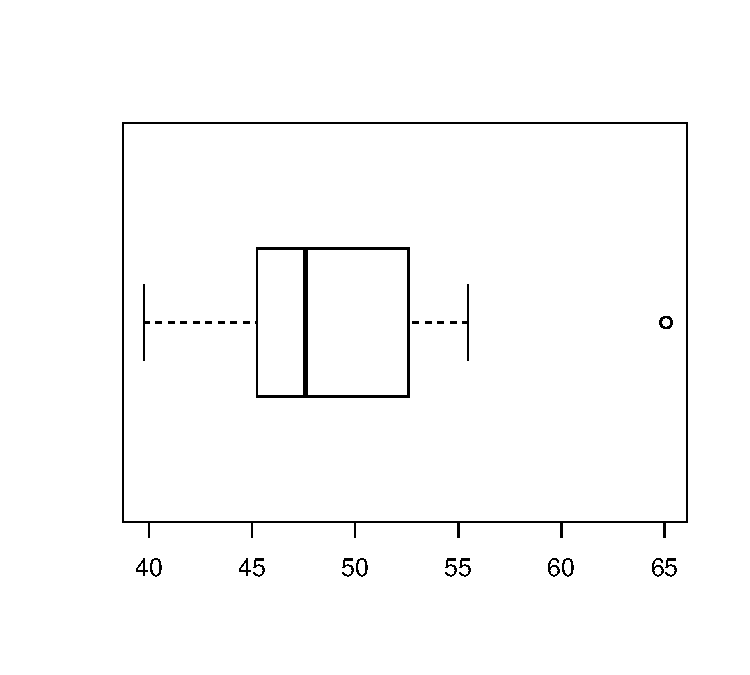
\includegraphics{CS01report_maressa_files/figure-latex/plot-1.pdf}

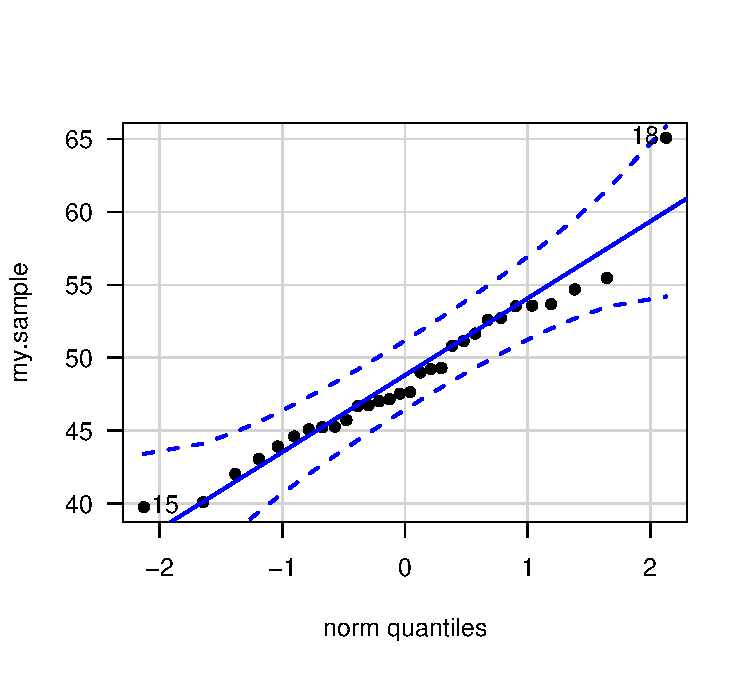
\includegraphics{CS01report_maressa_files/figure-latex/plot1-1.pdf}

\begin{verbatim}
## [1] 18 15
\end{verbatim}

Pela análise do boxplot e do gráfico quantil X quantil, verifica-se que,
embora o valor máximo observado (65.08) apresenta-se como um outlier no
boxplot, ele não interfere na normalidade dos dados. Sendo assim, é
possível prosseguir com as análises estatísticas que serão apresentadas
nas seções a seguir.

\hypertarget{resultados}{%
\section{Resultados}\label{resultados}}

\hypertarget{validacao-das-premissas}{%
\subsection{Validação das premissas}\label{validacao-das-premissas}}

\hypertarget{teste-do-custo-medio}{%
\subsection{Teste do custo médio}\label{teste-do-custo-medio}}

\hypertarget{teste-da-variancia-do-custo}{%
\subsubsection{Teste da variância do
custo}\label{teste-da-variancia-do-custo}}

\hypertarget{analise-estatistica}{%
\section{Análise Estatística}\label{analise-estatistica}}

\hypertarget{teste-sobre-a-media-do-custo}{%
\subsection{Teste sobre a média do
custo}\label{teste-sobre-a-media-do-custo}}

\hypertarget{calculo-do-tamanho-amostral}{%
\subsubsection{Cálculo do tamanho
amostral}\label{calculo-do-tamanho-amostral}}

\hypertarget{teste-de-hipoteses}{%
\subsubsection{Teste de Hipoteses}\label{teste-de-hipoteses}}

\hypertarget{calculo-do-intervalo-de-confianca}{%
\subsubsection{Calculo do intervalo de
confianca}\label{calculo-do-intervalo-de-confianca}}

\hypertarget{validacao-das-premissas-1}{%
\subsubsection{Validaçao das
premissas}\label{validacao-das-premissas-1}}

\hypertarget{teste-sobre-a-variancia-do-custo}{%
\subsection{Teste sobre a variância do
custo}\label{teste-sobre-a-variancia-do-custo}}

\hypertarget{teste-de-hipoteses-1}{%
\subsubsection{Teste de Hipoteses}\label{teste-de-hipoteses-1}}

\hypertarget{calculo-do-intervalo-de-confianca-1}{%
\subsubsection{Calculo do intervalo de
confianca}\label{calculo-do-intervalo-de-confianca-1}}

\hypertarget{validacao-das-premissas-2}{%
\subsubsection{Validaçao das
premissas}\label{validacao-das-premissas-2}}

\hypertarget{discussao-e-conclusoes}{%
\section{Discussão e Conclusões}\label{discussao-e-conclusoes}}

\hypertarget{divisao-das-atividades}{%
\section{Divisão das Atividades}\label{divisao-das-atividades}}

Victor - Reporter Maressa - Coordenadora Gilmar - Verificador e Monitor

\hypertarget{referencias}{%
\section{Referências}\label{referencias}}


\end{document}
